% !TEX program = xelatex
\documentclass[a4paper]{article}
\usepackage{amsmath}
\usepackage{amsthm}
\usepackage[left=1.8cm,right=1.8cm,top=2.2cm,bottom=2.0cm]{geometry}
\usepackage{ctex}
\usepackage{enumerate}
\usepackage{fancyhdr}
\usepackage{xpatch}
\usepackage{graphicx} 
\usepackage{float} 
\usepackage{subfigure} 
\usepackage{amsfonts}
\usepackage{mathtools}
\usepackage{framed}
\usepackage{multicol}
\usepackage{listings}
\usepackage{hyperref}
\usepackage{tikz}
\usetikzlibrary{automata,positioning}
\theoremstyle{definition}
\newtheorem*{solution*}{\textbf{Solution:}}
\newtheorem*{proof*}{\textbf{Proof:}}
\newtheorem{theorem}{Theorem}[subsection]
\newtheorem{definition}{Definition}[subsection]
\newtheorem{lemma}{Lemma}[subsection]
\makeatletter
\usepackage{listings}% http://ctan.org/pkg/listings
\lstset{
  basicstyle=\ttfamily\tiny,
  mathescape,
}
\AtBeginDocument{\xpatchcmd{\@thm}{\thm@headpunct{.}}{\thm@headpunct{}}{}{}}
\makeatother

\pagestyle{fancy}
\renewcommand{\baselinestretch}{1.15}
\usepackage[scaled=0.85]{FiraMono}

\lstset{basicstyle=\ttfamily, keywordstyle=\bfseries}
\usepackage{paralist}
\let\itemize\compactitem
\let\enditemize\endcompactitem
\let\enumerate\compactenum
\let\endenumerate\endcompactenum
\let\description\compactdesc
\let\enddescription\endcompactdesc

% shorten footnote rule
\xpatchcmd\footnoterule
  {.4\columnwidth}
  {1in}
  {}{\fail}

\title{CS 131 Compilers: Discussion 9: Naive Codegen}
\author{\textbf{杨易为}~~\textbf{吴凌云}~~\textbf{樊雨鑫} \\ \texttt{ \{yangyw,wuly2,fanyx\}@shanghaitech.edu.cn}}


\begin{document}
\maketitle
\section{Scope}
From today on, we steps into a new topic: semantic. We cast analysis on the grammar from CFG and do as many checks as possible, during which we mark something like type, scope and runtime garbage collector so that they can do better in runtime.
\subsection{Dynamic Scoping}
A global identifier refers to the identifier associated with the most recent environment, and is uncommon in modern languages. In technical terms, this means that each identifier has a global stack of bindings and the occurrence of a identifier is searched in the most recent binding.

\begin{lstlisting}[language=C]
/* Since dynamic scoping is very uncommon in the familiar languages, we consider the 
 * following pseudo code as our example. It prints 20 in a language that uses dynamic
 * scoping. */ 
int x = 10;
// Called by g()
int f() {
   return x;
} 
// g() has its own variable named as x and calls f()
int g() {
   int x = 20;
   return f();
}
main() {
  printf(g());
}
\end{lstlisting}
\subsection{Lexical Scoping}

\textbf{Scoping} refers to the issue of matching \href{https://docs.python.org/zh-cn/3.9/reference/compound_stmts.html#class-definitions}{identifier declarations} with its Uses. The \textbf{Scope} of an identifier is the portion of a program where it is accessible.
\begin{enumerate}
  \item Same identifier may refer to different things in different portions.
  \item Different scopes for same identifier \textbf{Do Not} overlap.
  \item Usually, search for \textbf{local} definition first, and if not found, goto its parent Scope.
\end{enumerate} 

\subsubsection{Python Scoping}

In python, we have 4 kinds of scopes and their life cycle, which is called \textbf{LEBG}. Notice that every scope maintain its namespace, which is literally a bunch of map of identifiers.

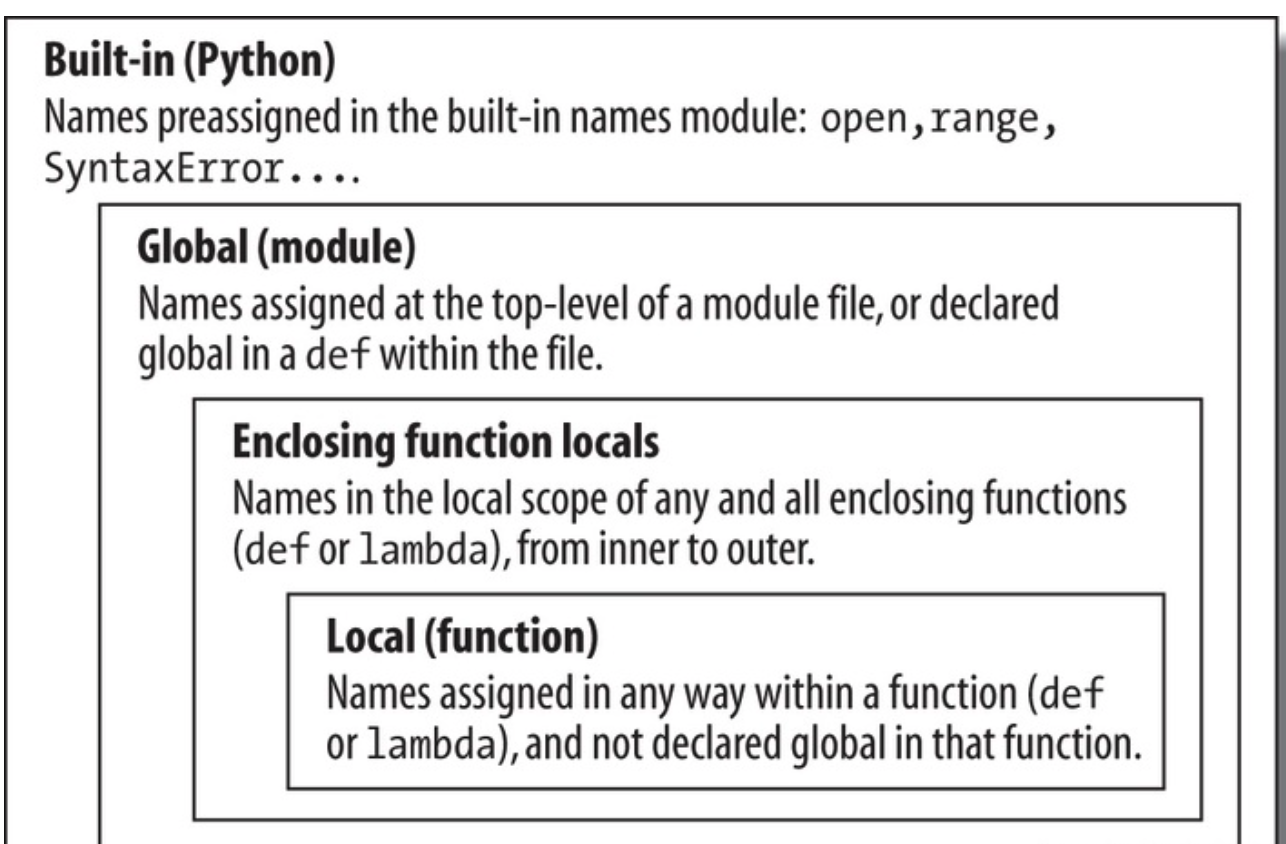
\includegraphics[width=10cm]{img/Snipaste_2021-04-24_02-41-32.png}
\begin{enumerate}
  \item \textbf{L}ocal scope,  that is, the temporary variables defined in the function, when the function ends, the life cycle of the variable ends.

  \item \textbf{E}nclosed (closure, the local scope of the nested parent function), that is, the local variables of the outer function of the closure, the end of the outer function, the end of the life cycle of the variable.
  \item \textbf{G}lobal (global variables), that is, variables defined at the module level, the module is destroyed, the life cycle of the variable will end.
  \item \textbf{B}ulit-in (built-in function) is the python interpreter, the virtual machine built-in variables.
\end{enumerate}

Here we put a benign testcases and adversarial testcases
\begin{enumerate}
  \item  The benign one
    \begin{lstlisting}
      +--------------------------+
      |        +---------------+ |
      | def foo|():            | |
      |   +----+               | |
      |   | x = 1              | |
      |   |          +-------+ | |
      |   | def inner|():    | | |
      |   |   +------+       | | |
      |   |   | return x + 1 | | |
      |   |   +--------------+ | |
      |   | x = 3              | |
      |   | print inner()      | |
      |   +--------------------+ |
      +--------------------------+
    \end{lstlisting}

  This inner is a closure(lambda function). The way closures are implemented in Python is to hold a pointer to an external namespace (which can be interpreted as a dictionary).
\\
  \textbf{Question:} What's the result of the following output?
\begin{lstlisting}
def make_averager():
    count = 0
    total = 0
    def averager(new_value):
        nonlocal count, total
        count += 1
        total += new_value
        return total / count
    return averager

averager = make_averager()
print(averager(10))
print(averager(11))
\end{lstlisting}
\textbf{Answer:}
\\
\\
\\
  \item The malicious one
\begin{lstlisting}[language=Python]
def f0(): // NameError: name 'a' has'nt been defined
  a = 123
  def g():
      exec("print(a)")
  g()

def f1(): // print("123\n123")
  a = 123
  def g():
      exec("print(a)")
      print(a)
  g()

def f2(): // NameError: name 'a' has'nt been defined
  a = 123
  def g():
      print(eval("a"))
  g()

def f3(): // print("123\n123")
  a=123
  def g():
      print(eval("a"))
      print(a)
  g()
  \end{lstlisting}
The \textbf{eval} is another story. The built-in \textbf{eval} function, which evaluates a string as a Python expression(运行字符串中存储的指令). The grammar is listed below.
\begin{lstlisting}
  eval(source[, globals[, locals]]) -> value
\end{lstlisting}
Where \textbf{source} is a Python expression or code object return by a function \textbf{compile()}, global is dictionary and locals is any mapped object. 

\end{enumerate}
\subsubsection{Doc is not enough, show me your code}

The \href{https://github.com/python/cpython/blob/3191391515824fa7f3c573d807f1034c6a28fab3/Python/clinic/bltinmodule.c.h#L326}{code} is from \href{https://en.wikipedia.org/wiki/CPython}{CPython}, a interpreter in C to speed up python.
\begin{lstlisting}[language=C]
static PyObject *
builtin_eval(PyObject *module, PyObject *const *args, Py_ssize_t nargs)
{
    PyObject *source;
    PyObject *globals = Py_None;
    PyObject *locals = Py_None;

    source = args[0];
    globals = args[1];
    locals = args[2];
/* ... Checks */
int r = _PyDict_ContainsId(globals, &PyId___builtins__);
if (r == 0) {
    r = _PyDict_SetItemId(globals, &PyId___builtins__,
                          PyEval_GetBuiltins());
}
if (r < 0) {
    return NULL;
}

if (PyCode_Check(source)) {
    if (PySys_Audit("exec", "O", source) < 0) {
        return NULL;
    }

    if (PyCode_GetNumFree((PyCodeObject *)source) > 0) {
        PyErr_SetString(PyExc_TypeError,
            "code object passed to eval() may not contain free variables");
        return NULL;
    }
    return PyEval_EvalCode(source, globals, locals);
}

PyCompilerFlags cf = _PyCompilerFlags_INIT;
cf.cf_flags = PyCF_SOURCE_IS_UTF8;
str = _Py_SourceAsString(source, "eval", "string, bytes or code", &cf, &source_copy);
if (str == NULL)
    return NULL;

while (*str == ' ' || *str == '\t')
    str++;

(void)PyEval_MergeCompilerFlags(&cf);
result = PyRun_StringFlags(str, Py_eval_input, globals, locals, &cf);
Py_XDECREF(source_copy);
return result;
}
\end{lstlisting}

\textbf{Problem:} What is the above code impls of scoping, evaluation at which time and how \textbf{eval()} interact with input strings?

\textbf{Answer}:
$$
\\
$$
\subsubsection{The Scope of Decorator}
When we analyze the calling process of a unknown procedure. The decorator in Python is to make the grammar nice and neat. If you work for Python Open Source community, you must have heard of \href{https://www.python.org/dev/peps/pep-0008/}{PEP8}. Utilizing Decorator and other grammar sweet is a good way, and also may give you a insight to understand others' reason of writing so. For a general view, a language is all about its grammar sweet.

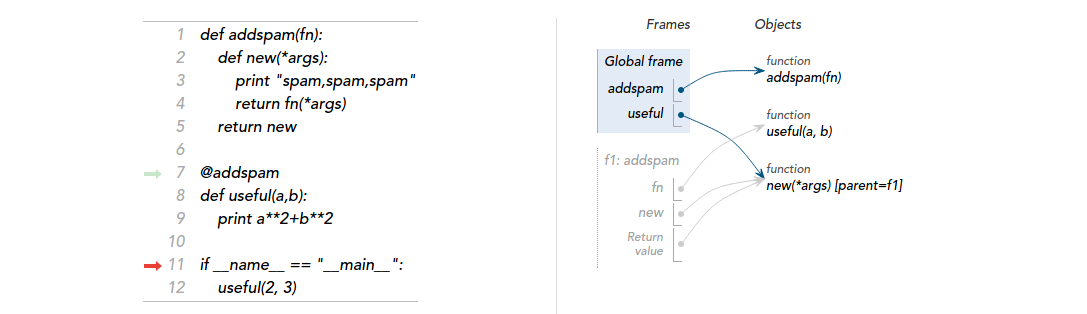
\includegraphics[width=15cm]{./img/b5674ca16f72af11d7a1c70602fbfe10_b.png}



\subsubsection{Make good use of Python Scoping}
\begin{lstlisting}[language=Python]
class IntermediateNumber(ABC):
  # class internal namespace, can be shared through the lifetime of the class
  numbers: ClassVar[List[int]]
  digits: int
  def __init__(self, number: Union[List[int], int], digits: int, from_natural: bool):
      self.digits = digits
      if from_natural:
          self.numbers = self.from_natural(number)
      else:
          # builtin function
          if isinstance(number, int): # convert int to List[int]
              numbers = [int(c) for c in str(number)]
          else:
              numbers = number
          # class function
          if not self.check(numbers):
              raise ValueError(f'number not valid: {numbers}')
          self.numbers = numbers
      if digits - 1 > len(self.numbers):
          self.numbers = [0] * (digits - 1 - len(self.numbers)) + self.numbers
  # internal function for stringify
  def __str__(self):
      return f'{self.__class__.__name__[:3]}({"".join(map(str, self.numbers))}){self.custom_str()}'
  # type checking, rhs is callable.
  def check(self, number: List[int]) -> bool:
      return True
  def __add__(self, rhs: IntermediateNumber):
      assert isinstance(self, rhs.__class__)
      return self.add(rhs)
  def __sub__(self, rhs: IntermediateNumber):
      assert isinstance(self, rhs.__class__)
      assert self.to_natural() >= rhs.to_natural()
      return self.sub(rhs)
  # rhs is callable.
  # generate from natural number
  @abstractmethod
  def from_natural(self, natural: int) -> List[int]:
      pass
  # convert back to natural number
  @abstractmethod
  def to_natural(self) -> int:
      pass
  @abstractmethod
  def add(self, rhs: IntermediateNumber):
      pass
  @abstractmethod
  def sub(self, rhs: IntermediateNumber):
      pass
\end{lstlisting}

Better for libraries' unit tests and fuzzing tests.

\subsubsection{Python interpretor is not as strong as you think}
Not every is picklable, a serialization technique when packing tedious python object. We need it because when we need to have multiprocessing or networking stuffs while because of GIL, python is too too too slow. What is not picklable?
The lambda functions along with functions and classes defined in the \_main\_ module, which is the function in the global scope or in a class function.

How to solve it?

Cloud-pickle.
\begin{lstlisting}[language=Python]
from .cloudpickle import (
    _extract_code_globals, _BUILTIN_TYPE_NAMES, DEFAULT_PROTOCOL,
    _find_imported_submodules, _get_cell_contents, _is_importable,
    _builtin_type, _get_or_create_tracker_id,  _make_skeleton_class,
    _make_skeleton_enum, _extract_class_dict, dynamic_subimport, subimport,
    _typevar_reduce, _get_bases, _make_cell, _make_empty_cell, CellType,
    _is_parametrized_type_hint, PYPY, cell_set,
    parametrized_type_hint_getinitargs, _create_parametrized_type_hint,
    builtin_code_type,
    _make_dict_keys, _make_dict_values, _make_dict_items,
)
\end{lstlisting}
\section{Type System}
A type is a set of values together with a set of operations on those values. A language's type system specifies which operations are valid for which types. 

\subsection{Type Inference(not interface in java/ts)}
Types of expressions and parameters need not be explicit to have static typing. With the right rules, might infer their types.

The appropriate formalism for type checking is logical rules of inference having the form. cool is a statically typed

\begin{lstlisting}[language=C]
  doh() : Int { (let i : Int <- h in { h <- h + 2; i; } ) };
\end{lstlisting}

Here the doh can be inferred as the type should be int even doh() does not have a type hint.
\subsection{Type Checking Rules}
Goal of type checking is to ensure that operations are used with the correct types, enforcing intended interpretation of values.

Notion of "correctness" often depends on what programmer has in mind, rather than what the representation would allow.

Most operations are legal only for values of some types
\begin{enumerate}
  \item Doesn’t make sense to add a function pointer and an integer in C
  \item It does make sense to add two integers
  \item But both have the same assembly language implementation: movl y, \%eax;  addl x, \%eax
\end{enumerate}

\subsection{Type System for a Toy Language}
Define a really easy typeof to connect with operational semantic for cool. we only will consider the following subset grammars.
\begin{verbatim}
  defn(I,T,[def(I,T)| _])
  defn(I, T, [def(I1,) | R]) :- dif(I, I1), defn(I, T, R).
  typeof(X, T, Env) :- defn(X, T, Env).
  \end{verbatim}
  \_ means “don’t care” or “wildcard”, $I$ is defined to have type $T$ if the environment list starts with such a definition, or if $I$ isn't the same as the identifier in the first def but matches the next suitable definition further down the list.
\begin{verbatim}
  e : ID | int
    | [ ((e ,)* e)?  ] /* list */
    | lambda ( ID , e )
    | e ’+’ e
    | e ’<<’ e
    | e ’//’ e
    | cast(e,e)
\end{verbatim}

Begin with two typing rules.
\begin{verbatim}
  typeof(X, int,) :- integer(X).
  typeof(X, T, Env) :- defn(X, T, Env).
\end{verbatim}

\begin{enumerate}
  \item Write a typing rule such that the type of an empty list is unbounded (e.g [\_]).
  
  \textbf{Answer:}
  
  \item  Write a typing rule such that the type of a list is [T], where all list elements are of type T.
  
  \textbf{Answer:}
  
  \item Write a typing rule such that the type of a lambda is $T1->T2$, where $T2$ is the returntype and $T1$ is the type X is bound to within the body of the lambda.

  \textbf{Answer:}
  
  \item Write a typing rule such that the type of $L + R$ isintwhenLandRare both of type int.
  
  \textbf{Answer:}

  \item Write a typing rule such that the type of $L // R$ is [T] whenLandRare both of type [T].
  
  \textbf{Answer:}
  \item Write a typing rule such that the type of $cast(L,R)$ is $T1 -> T2$ when L is of type $T1$ and R is of type $T2$.
  
  \textbf{Answer:}

\end{enumerate}

Then we can get the reverse opertaion to infer type using typeof:
\begin{enumerate}
  \item \begin{verbatim}
typeof(f << g, T, [def(f, int->[int]), def(g, int)]).
  \end{verbatim}
  
  \textbf{Answer:}
  \item \begin{verbatim}
typeof(lambda(x, x // x) << [1], T, []).
  \end{verbatim}

  \textbf{Answer:}
  \item \begin{verbatim}
typeof(lambda(x, x + x) << 1, T, []).
  \end{verbatim}

  \textbf{Answer:}
  \item \begin{verbatim}
typeof(lambda(x, x + x) + 1, T, []).
  \end{verbatim}

  \textbf{Answer:}
  \item \begin{verbatim}
typeof(lambda(x, x // x) << [lambda(x, x // x)], T, []).
  \end{verbatim}

  \textbf{Answer:}
  \item \begin{verbatim}
typeof(lambda(x,lambda(y, cast(x,y))) << [lambda(x,lambda(y, cast(x,y)))],T, []).
  \end{verbatim}

  \textbf{Answer:}

\end{enumerate}


\subsection{Type Unification}
To unify two type expressions is to find substitutions for all type variables that make the expressions identical. This technique will be useful for PA3 and PA4, or you will not pass all the testcases. The algorithm that follows treats type expressions as objects (so two type expressions may have identical content and still be differ- ent objects). All type variables with the same name are represented by the same object. It generalizes binding by allowing all type expressions (not just type variables) to be bound to other type expressions.

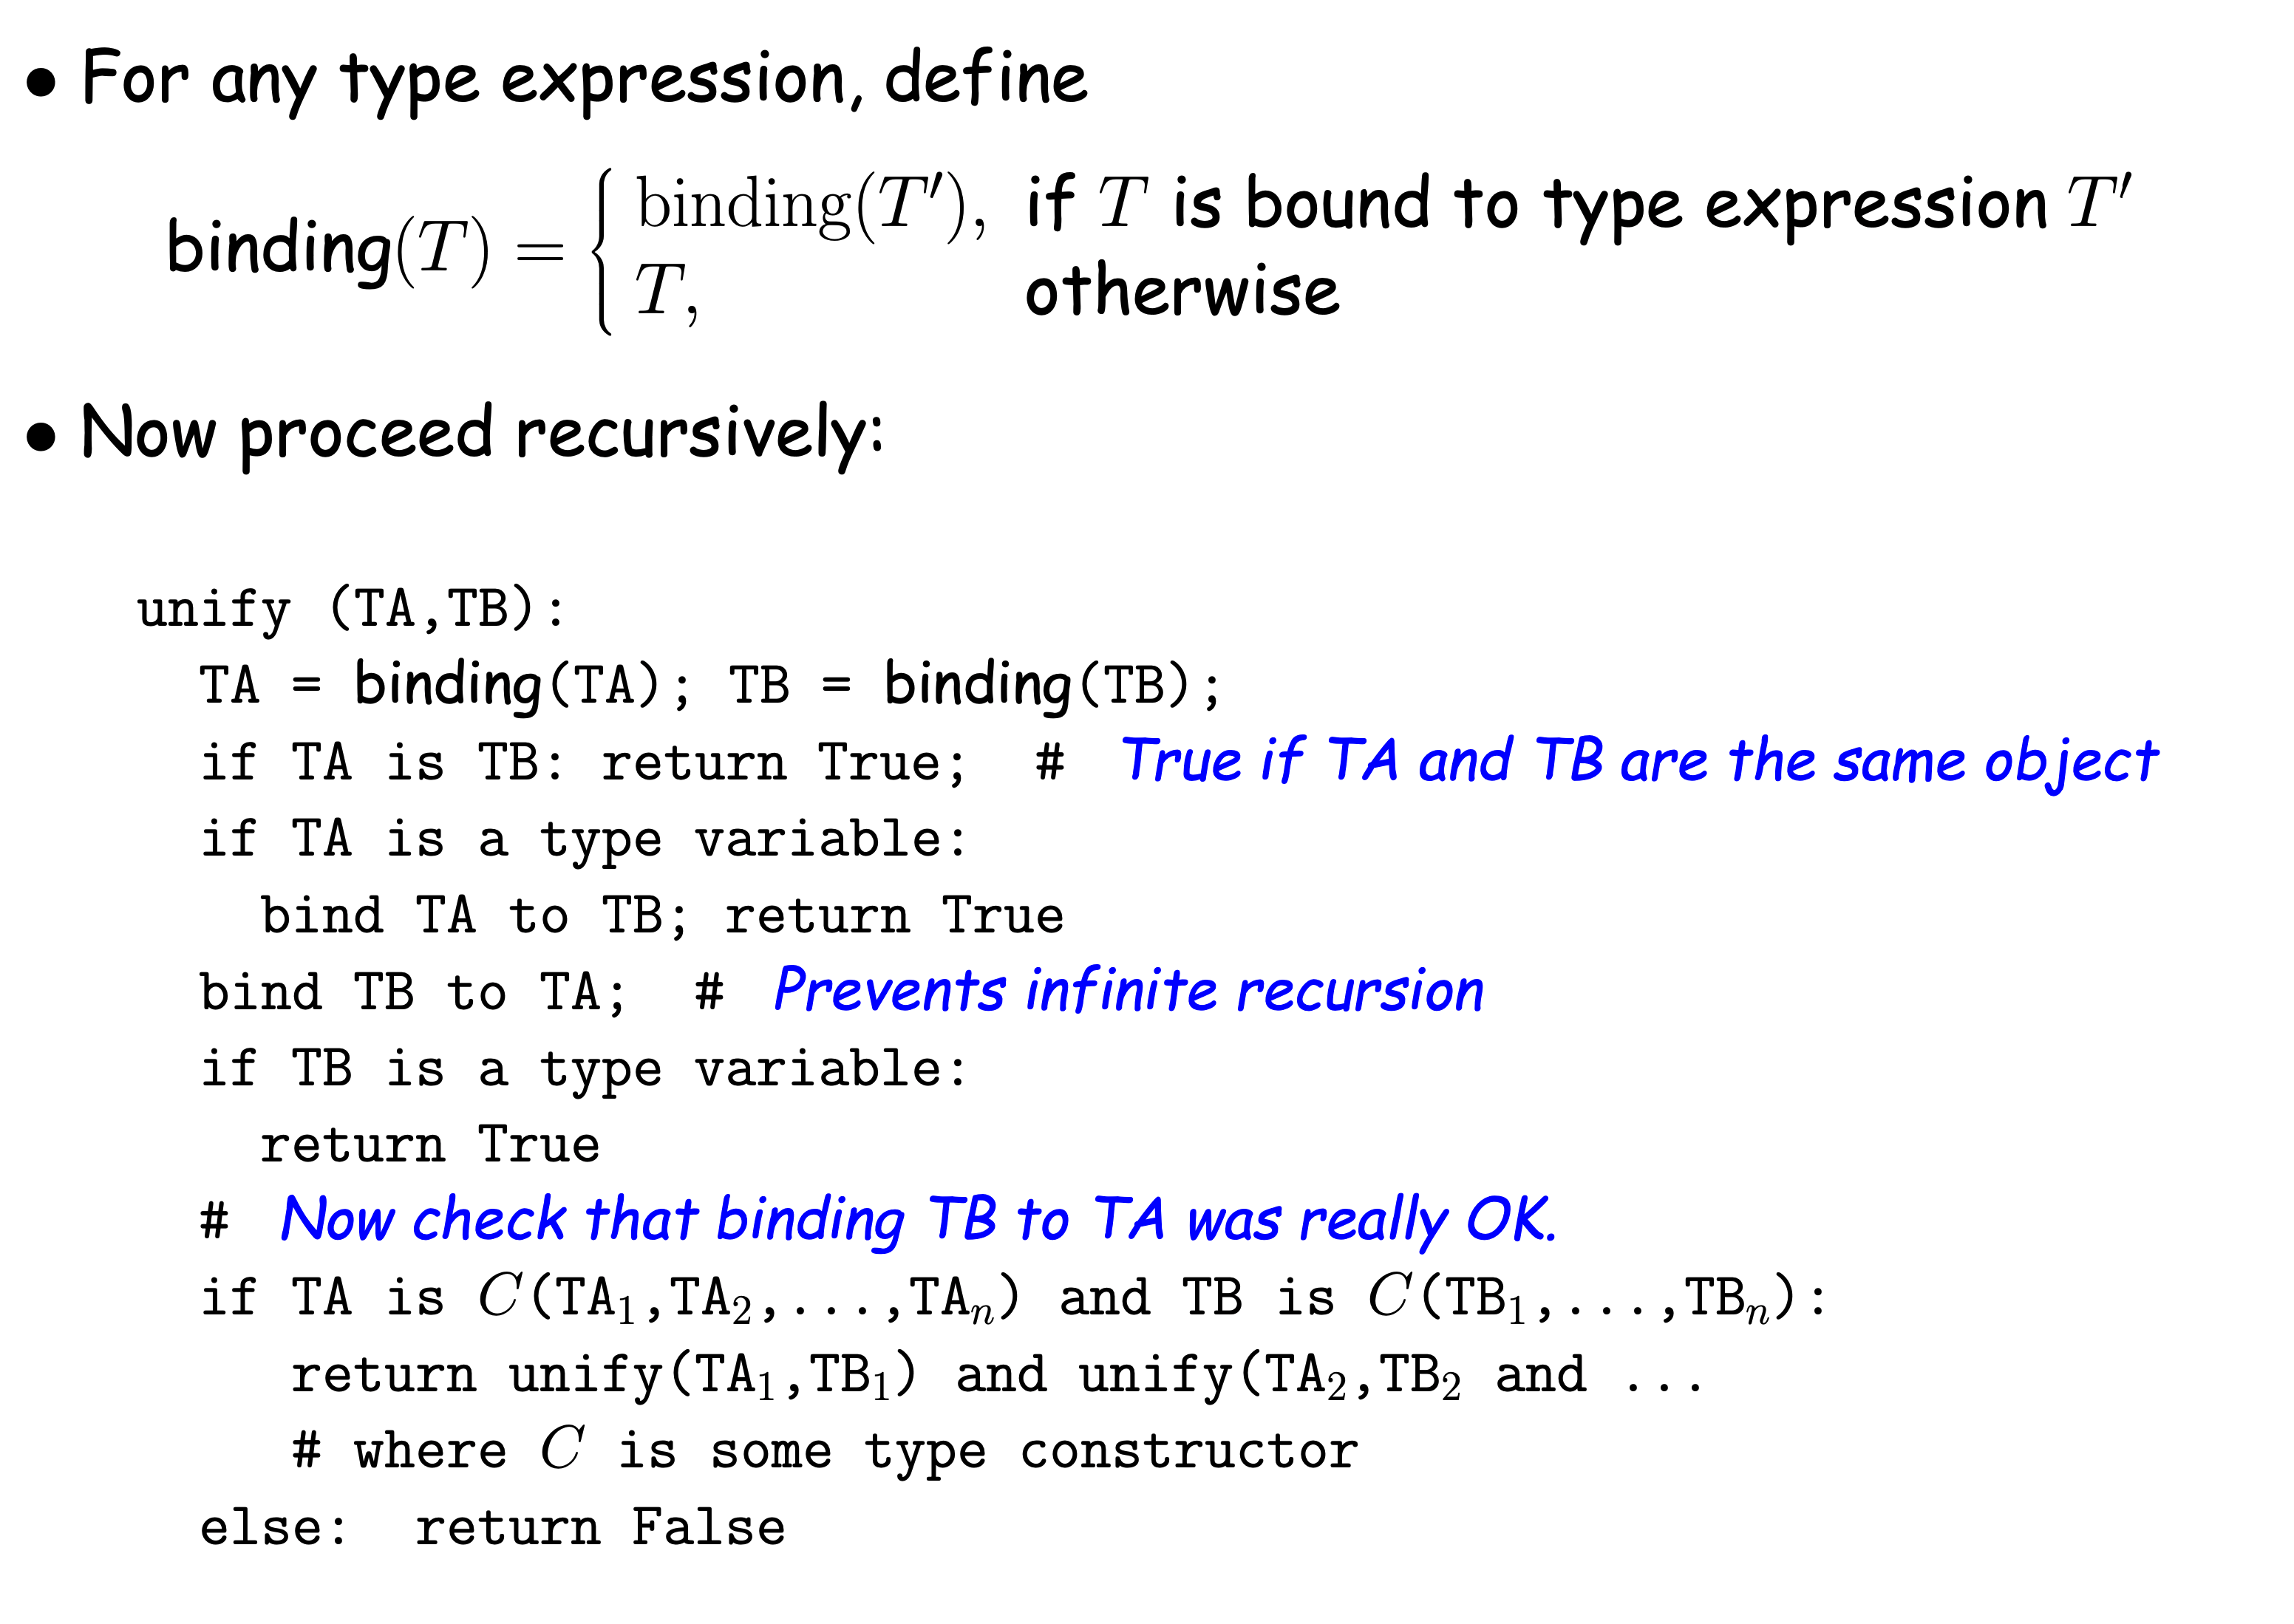
\includegraphics[width=10cm]{img/Snipaste_2021-05-08_04-55-14.png}
\end{document}
